\subsection{Structure of the section}
Overview stating the goals we want to convey though the experiment section. The what and how of the experiments.
\section*{Experiments}
\subsubsection*{Overview}
In this chapter we perform various qualitative and quantitative evaluations to showcase a comprehensive performance comparison of our method to others. All the experiments are conducted in the in-house built simulator described in Section \ref{section}. There are a lot of choices regarding methods and features that has been made, and we try to evaluate each of these choices against the existing work.\\
The first subsection provides a comparison among our IRL method, a classical agent and a RL based agent trained in similar setting using a simple yet dense hand-crafted reward function. This helps in demonstrating the difference in performance of agents coming from different training methods.\\
 Feature representations play a vital role in an IRL pipeline and so, the following section compares the performance of IRL agents trained in similar setting but different feature representations.\\
This is followed by a set of experiments to evaluate the generalizability of our setup, where the performance of an agent is compared between a known and an unknown environment. Here "known" is defined as the environment from which the expert demonstrations have been collected.\\

Getting tricky scenarios that help showcase the subtle qualitative aspects of a navigating agent from real-world video might be difficult and indeed with the time and effort spent scrolling through the videos to find these are hard, so we also generate some synthetic scenarios to check some of the specific, more advanced qualitative behaviors of the IRL and how that differs to that of the RL.

The last subsection, looks into the reward function: the second, and unfortunately, in most of the cases, ignored part of the equation. We try to visualize and interpret the reward function in an attempt to get a better insight into the functioning of our agent.

\subsubsection*{Description of the scenario}
To train our agent we select demonstrations from the UCY university students dataset \cite{ucy-dataset-university-students}. It consists of trajectories of 430 different pedestrians on a relatively busy area captured over a time span of 3 minutes and 37 seconds. The video is captured at 25 fps resulting in a total of 5400 frames. The length of the trajectories vary from $the min$  to $the max$ with an average of 406 frames per trajectory. 
\begin{figure}
	\caption {Distribution of pedestrian trajectory length}
\end{figure}
There are a few key properties that makes this environment challenging: dense crowd, open space so lack of any constrain offered by spaces like narrow pathways, as because open space pedestrians(obstacles) can and does come from different directions making the process of negotiating such crowds rather challenging. 

%\begin{table}
%	\caption {Table containing useful information on the what is useful}
%	\label{university-students-stats}
%		\begin{center}
%		\renewcommand{\arraystretch}{1.3}
%		\begin{tabular}{|c|c|}
%			\hline
%			Property  & Value \\
%			\hline
%			Number of pedestrians &    \\
%			Avg trajectory length &  \\
%			 & $\theta > 90\degree$\\
%			
%			Medium & otherwise \\
%			\hline
%		\end{tabular}
%	\end{center}
%\end{table} 
\subsubsection*{Description of the training parameters?}

The MEDIRL pipeline is run for 100 epochs. The AC2 \cite{ac2} training for the inner loop is run for a predefined fixed number of episodes where an episode terminates when the agent reaches the goal, hits an obstacle or exceeds a predefined maximum number of frames per episode. Both the policy and reward networks have a simple architecture with a single 256 dimensional hidden node with exponential linear unit (ELU) \cite{exponential-linear-unit} as the activation function and adaptive moment estimation (Adam) \cite{adaptive-moment-estimation} as the choice of optimizer. The learning rate for the policy and reward network are set to $0.001$ and $0.0005$ respectively.


\subsubsection*{Description of the metrics used}
%What do we want to show? 
%\begin{enumerate}
%	\item Justify the use of IRL over RL or traditional methods.
%	\item Establish the superiority of the feature representation over other
%	\item Show that the smoothing affects the performance of the agent in a positive way.
%	\item Show the generalizability of the method. (Compare the performance metrics of the agent in the two different scenarios.)
%	\item Another benefit of IRL is the availability of the reward network. Visualization and comprehension of the reward network. 
%\end{enumerate}
%How do we show?
%
%To test the generalization capabilities of our method we train on the expert demonstrations from lone of the video and test it on data from different scenarios.

%\begin{itemize}
%        \item Training and testing on the same annotation file.
%        \item Training and testing on different annotation files.
%        \item Testing on custom scenarios.
%\end{itemize}
To get a comprehensive comparison of the performance of the agents, we compare them among different metrics, each capturing a unique characteristic of the navigation behavior exhibited by the agent. The metrics are described below:
\begin{itemize}
        \item \textbf{Reaching the goal:} The ability to reach a goal from a given position is one of the fundamental criteria to measure the performance of a navigating agent. It is calculated as the percentage of runs per 
        \item \textbf{Distance to displacement ratio:} This metric captures the efficiency of the path an agent takes to move between two points. It is calculated as the ratio between the euclidean distance between the two points and the distance traveled by the agent to move between the two. So, for two agents moving from the same start and endpoints, given both of them are successful in reaching the goal, the agent taking a more direct path, is rated better than the other. (The results are shown in the form of histogram plots)
        \item \textbf{Minimum distance over time graphs:} Indicates the minimum distance maintained by an agent throughout its entire trajectory. It can be thought of as a measure of how 'dangerously' or 'cautiously' an agent behaves while interacting with neighboring obstacles. (line graphs over time frame)
        \item \textbf{Avg smoothness:} Trajectories traced by people are smooth with rare occurrences of drastic change in the heading direction. This metric measures how much an agent changes its heading direction, thus the smoothness of its trajectory while negotiating obstacles or navigating in general. (bar plots with error bars.)
        \item \textbf{Drift analysis plots: }This performs a direct comparison between the trajectory taken by an agent and the trajectory followed by the pedestrian, and is calculated as the MSE between the points on the trajectory of the agent and the pedestrian(ground truth)at each time frame. It is a measure of how much the trajectory traced by an agent conforms to the trajectory traced by the actual pedestrian when subjected to similar conditions. (line graphs with error bars)
        \item \textbf{Traced trajectory of multiple agents for a particular pedestrian:} Primarily a visual tool to see how an agent performs in comparison to the ground truth.
\end{itemize}

\section*{Results and discussion}
\subsection*{Testing the performance against other methods}
Here we compare an agent trained using our IRL pipeline to two different agents: a data driven RL agent and a model based potential-field controller. The RL agent is trained in the same environment as the IRL using similar training hyper-parameters and network architecture with a dense reward function shown in Table  \ref{table:reward-function-summarization}.
\begin{table}
	\caption{Summary of reward function for RL agent}
	\begin{center}
		\renewcommand{\arraystretch}{1.3}
		\begin{tabular}{|c|c|}
		\hline
		Condition & Reward assigned \\
		\hline
		Reach goal & 1 \\
		Hit obstacle & -1 \\
		Move towards goal & $0.01 \times \text{length of the step}$ \\
		Move away from goal & $ -0.01 \times \text{length of the step}$\\
		\hline
		\end{tabular}
	\end{center}
	\label{tab:reward-function-summarization}
\end{table}\\
\vspace{5cm}
The implementation of the potential field controller is based on \cite{khatib-potential-field}.\\  
\begin{figure}
	\centering
	\caption{Reaching the goal metric comparing the performance of RL v PF v IRL}
		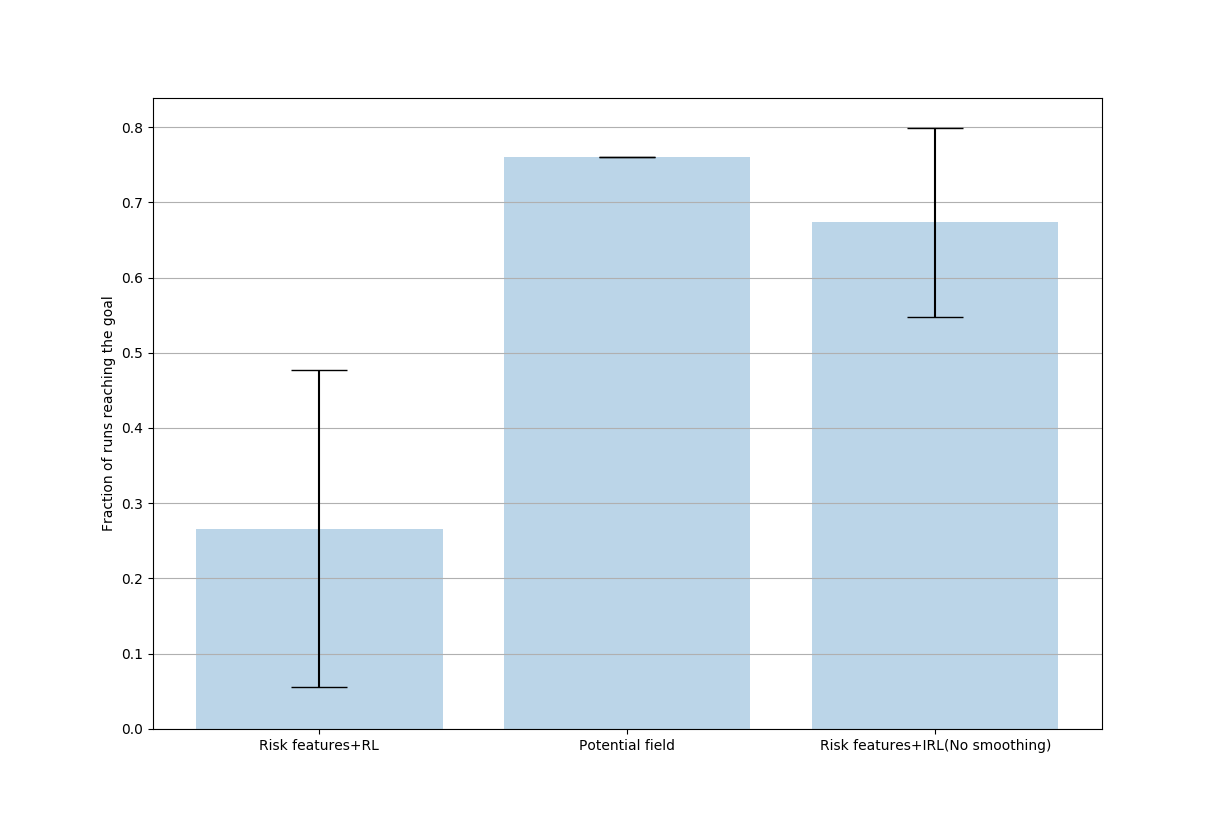
\includegraphics[width=0.6\linewidth]{plots/inter_method/goal_reached.png}
	\label{fig:inter-method-reach-goal}
\end{figure}\\
In Figure \ref{image1} we see that
\begin{figure}
	\centering
	\caption{Comparison of the number of runs in which an agents hits a pedestrian}
	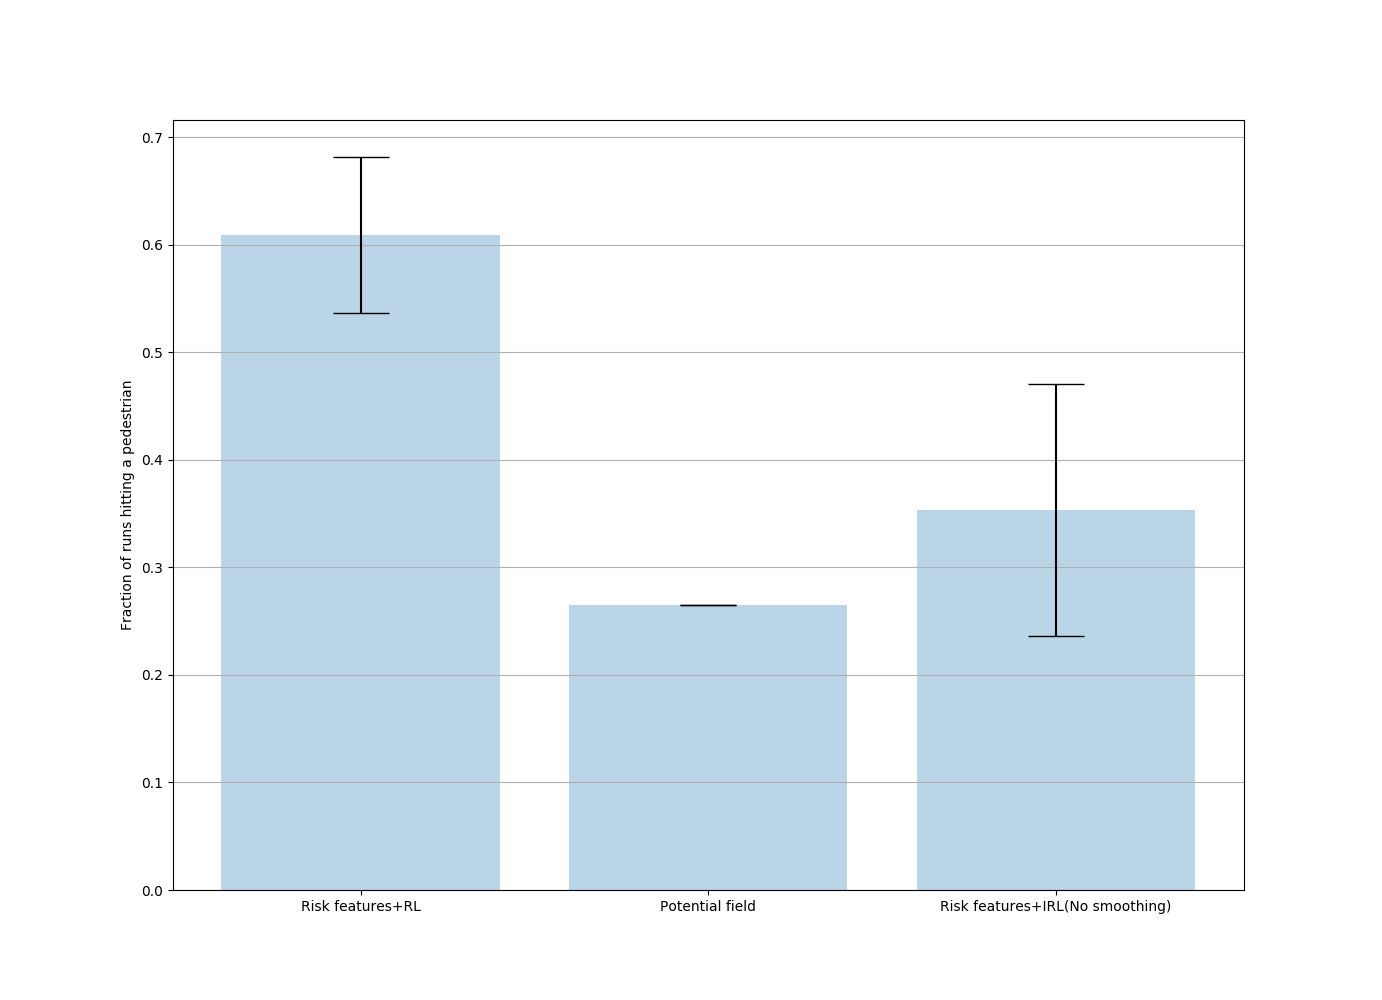
\includegraphics[width=0.6\linewidth]{plots/inter_method/hit_pedestrian.png}
	\label{fig:inter_method-hit_pedestrian}
\end{figure}

\begin{figure}
	\centering
	\caption{Total change in orientation of different agents.}
	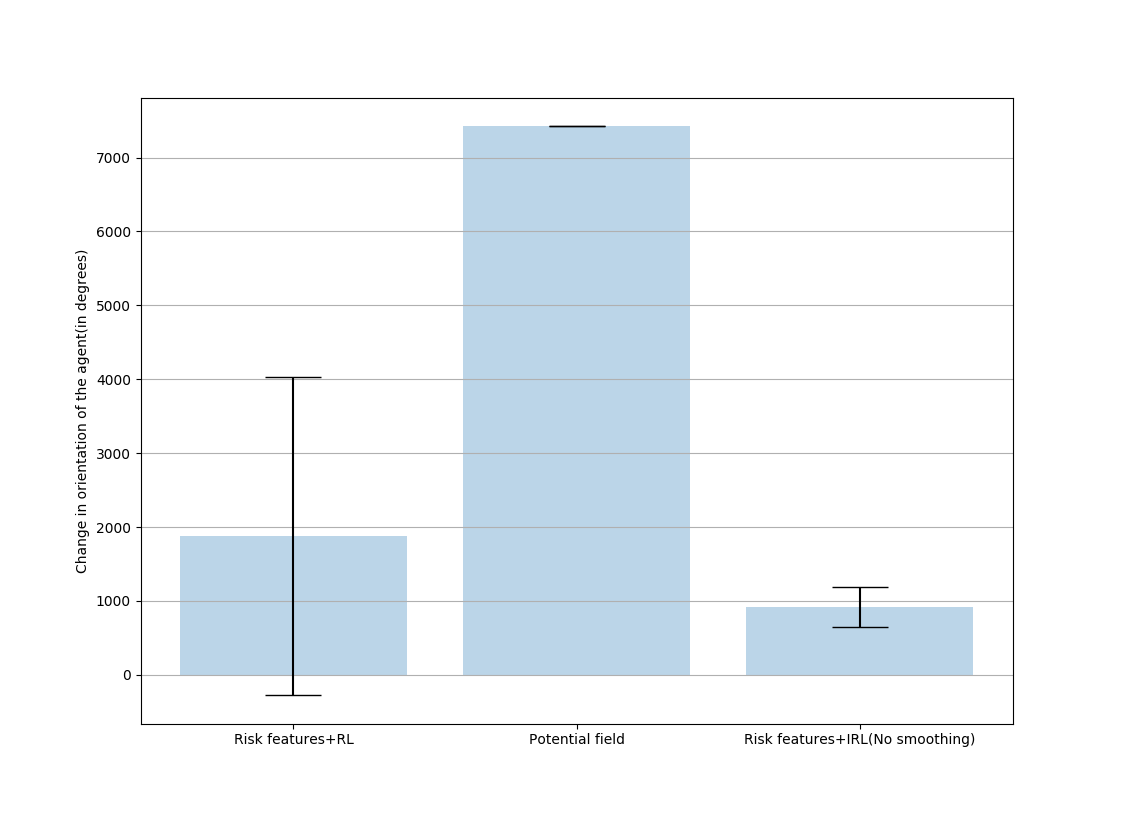
\includegraphics[width=0.6\linewidth]{plots/inter_method/change_in_orientation_total.png}
	\label{fig:inter_method-change_in_orientation_total}
\end{figure}


\begin{figure}
	\centering
	\caption{Average change in orientation per frame of different agents}
	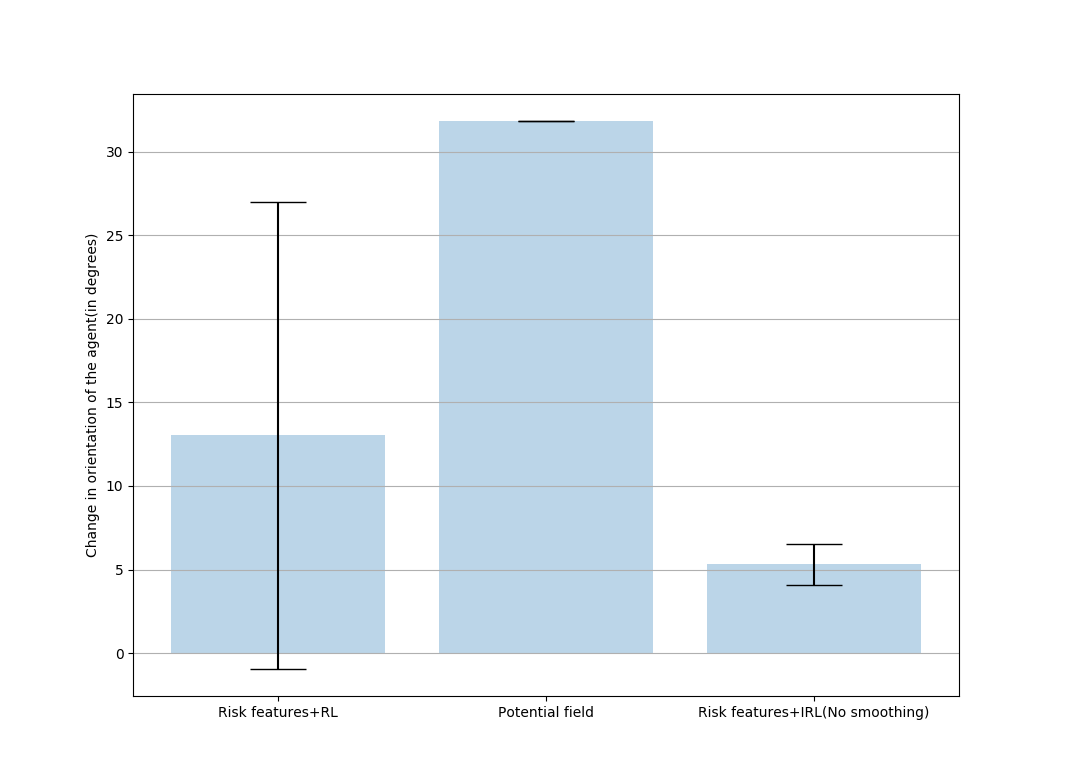
\includegraphics[width=0.6\linewidth]{plots/inter_method/change_in_orientation_avg.png}
	\label{fig:inter_method-change_in_orientation_avg}
\end{figure}


\begin{figure}[!htbp]
	\centering
	\caption{Drift analysis}
	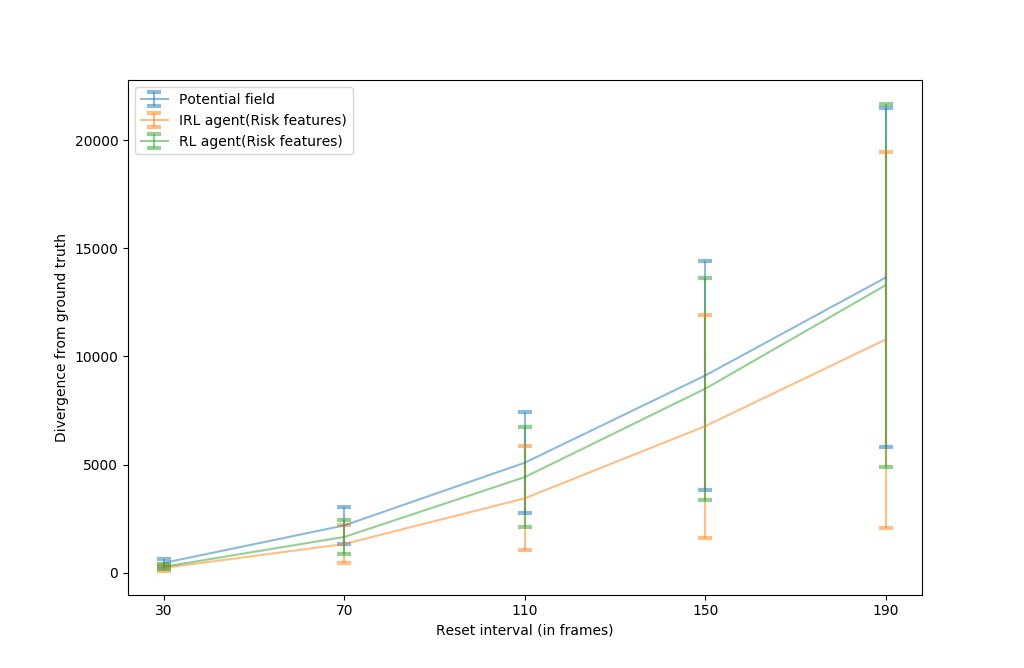
\includegraphics[width=0.6\linewidth]{plots/inter_method/drift_pf_irl_rl.png}
	\label{fig:inter_method-drift_analysis}
\end{figure}

\subsection*{Testing the performance of our feature representation against pre existing ones}
\subsubsection*{Description of the other feature extractors}
To test for the efficacy of our proposed risk-based feature representation, we test agents trained on our training pipeline with different existing feature representations. For this, we use feature representations proposed in \cite{fahadLearningHowPedestrians2018a} and \cite{vasquezInverseReinforcementLearning2014a} with some minor modifications and adjustments.\\
\textbf{Fahad}\\
Due to an underwhelming performance of the originally proposed SAM feature representation from \cite{fahadLearningHowPedestrians2018a} in our environmental setup, we substitute the part of the feature representation accommodating the goal information originally proposed by the authors with our goal representation. We call this modified version the 'Goal conditioned SAM'.
\textbf{Vasquez}\\
We use the feature sets $\mathcal{F}_1$, $\mathcal{F}_2$ and $\mathcal{F}_3$ from \cite{vasquezInverseReinforcementLearning2014a} and as before substitute their goal information with our goal information.\\
\textbf{Discuss the results}

\begin{figure}[!htbp]
	\centering
	\caption{text}
	\label{feature-rep-comparison-reach-goal}
	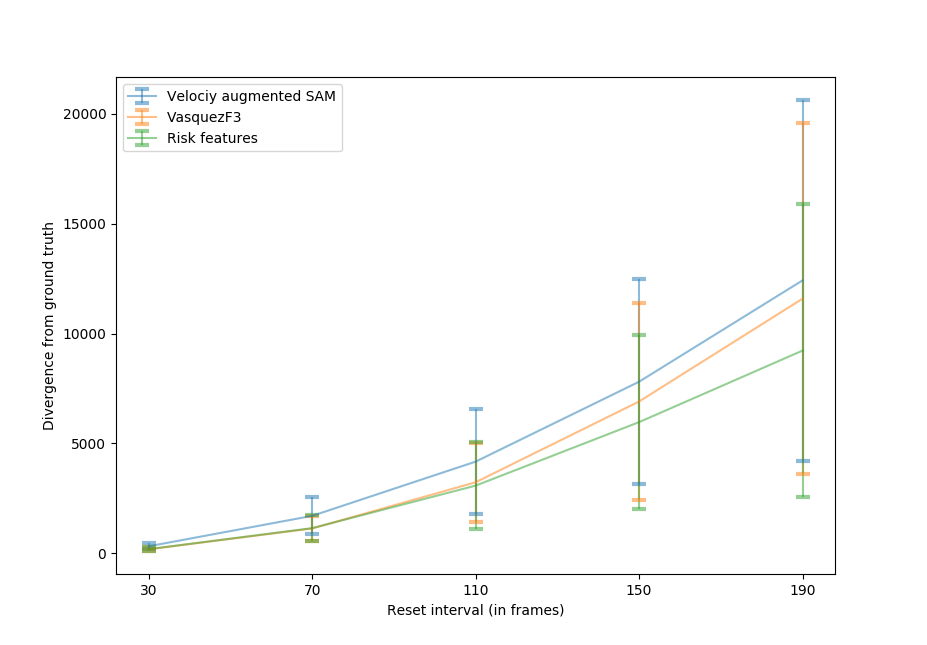
\includegraphics[width=0.7\linewidth]{plots/inter_IRL/drift_analysis_irl.png}
\end{figure}




\subsection*{Testing for generalization}
Description of the other dataset.
Discussion of the results.
\subsection*{Testing on custom scenarios}

\subsection*{Understanding the reward function}

